\scanpage{132}

In this example, one sees at once that\deleted{e} there is on $C$ a commutativity \unsure{constraint} compatible with the other data if and only if $U$ is commutative that is to say $G$ is commutative, and that the said constraints correspond \inserted{then} to the functions $: G\unsure{x|\times}G\handwritten{\unsure{\rightharpoondown|\rightarrow|-}} k^{\handwritten{*}}$ which are bilinear and antisymmetric. In the case where the $H^{2}(G,k^{\handwritten{\unsure{*|'}}})$ is \inserted{geometrically} zero (for example $G$ cyclic \deleted{and $k$ algebraically closed}) one therefore sees that for every nonzero choice of $\handwritten{\sigma}$, one has a commutativity constraint for which there is no fiber functor compatible with the said constraint (and the others over any extension of $k$. One may think of getting out of it by finding at least graded fiber functors compatible with all the constraints but one already sees that this is impossible if $k$ of characteristic two (where there is n\rlap{q}o diff\unsure{\rlap{a}e|e}rence between the existence of the one and the other type of fiber functor, graded or not); and probably the analysis must show that one has the same negative result in every characteristic. Note however in these examples one could at least, by modifying the given commutativity constraint, find one which admits a fiber functor compatible with the said constraint. There would therefore be reason to give an example of a $\unsure{\otimes|\Omega}$-category definable by a bialgebra\deleted{\unsure{s}}, admitting a commutativity constraint (compatible with the rest) but no commutativity const\rlap{a}raint for which one can \rlap{f}f\rlap{o}ind a fiber functor (graded if need be)\unsure{;|:}over any extension of the given field.

\handwritten{With the notation of number 11, we shall therefore need 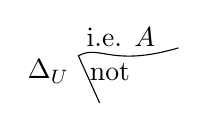
\begin{tikzpicture}[baseline=(du.base),x=1cm,y=1cm]
\node[inner sep=0] (du) at (0,0) {$\Delta_U$};
\node[anchor=west,inner sep=0] at (.52,0) {not};
\node[anchor=south,inner sep=0] at (.92,.31) {\inserted{i.e. $A$}};
\draw (1.65,.3) .. controls (.8,.05) and (.65,.35) .. (.38,.2) -- (.65,-.4);
\end{tikzpicture} commutative\inserted{\unsure{seen!|u.!}}, and $U$ noncommutative (otherwise the existence of $\sigma$ would imply the commutativity of $\Delta$\unsure{]|)}.}
% archive sheet number: 131
